\documentclass[a4paper, 12pt, twoside, openany]{article}

% Pakiety
\usepackage[utf8]{inputenc}
\usepackage[T1]{fontenc}
\usepackage[polish]{babel}
\usepackage[hidelinks]{hyperref} % Hiperłącza bez ramek
%\usepackage{hyperref} % Hiperłącza
\usepackage{amsmath, amssymb} % Pakiety matematyczne
\usepackage{mathtools}
\usepackage{graphicx} % Obsługa grafiki
\graphicspath{{../images/}}
\usepackage{enumitem}
%\usepackage{fontspec}
\usepackage{float}
\usepackage[font=footnotesize,labelfont=bf]{caption}
\usepackage{setspace}
\usepackage{geometry} % Ustawienia marginesów
\geometry{
    inner=20mm, % margines wewnętrzny
    outer=20mm, % margines zewnętrzny
    top=25mm,   % margines górny
    bottom=25mm % margines dolny
}
\usepackage{xcolor}   % Pakiet do kolorów
\usepackage{listingsutf8} % Pakiet do listingu kodu
\lstdefinestyle{mystyle}{
    inputencoding=utf8,           % Kodowanie UTF-8
    extendedchars=true,           % Obsługa znaków spoza ASCII
    basicstyle=\ttfamily\footnotesize,   % Styl podstawowy
    language=Matlab,              % Język kodu
    keywordstyle=\bfseries\color{blue}, % Styl słów kluczowych
    commentstyle=\itshape\color{green!50!black}, % Styl komentarzy
    stringstyle=\color{red},      % Styl tekstu w cudzysłowach
    numbers=left,                 % Numeracja linii po lewej stronie
    numberstyle=\color{gray},     % Styl numerów linii
    frame=single,                 % Ramka wokół kodu
    breaklines=false,             % Zawijanie linii
    backgroundcolor=\color{gray!10}, % Kolor tła
    tabsize=2,                    % Wielkość tabulacji
    showstringspaces=false,        % Ukrywanie spacji w ciągach tekstowych
    literate={ą}{{\k{a}}}1
             {Ą}{{\k{A}}}1
             {ć}{{\'{c}}}1
             {Ć}{{\'{C}}}1
             {ę}{{\k{e}}}1
             {Ę}{{\k{E}}}1
             {ł}{\l}1
             {Ł}{\L}1
             {ń}{{\'{n}}}1
             {Ń}{{\'{N}}}1
             {ó}{{\'{o}}}1
             {Ó}{{\'{O}}}1
             {ś}{{\'{s}}}1
             {Ś}{{\'{S}}}1
             {ź}{{\'{z}}}1
             {Ź}{{\'{Z}}}1
             {ż}{{\.{z}}}1
             {Ż}{{\.{Z}}}1
}
\lstset{style=mystyle}

\renewcommand{\figurename}{Rys}

\newcommand{\y}{\mathbf{y}}
\newcommand{\I}{\mathbf{I}}
\newcommand{\A}{\mathbf{A}}
\newcommand{\f}{\mathbf{f}}
\renewcommand{\b}{\mathbf{b}}

\newcommand{\tytul}{Rozwiązywanie układów równań różniczkowych zwyczajnych}
\newcommand{\autor}{Wiktor Murawski}
\newcommand{\uczelnia}{Politechnika Warszawska}
\newcommand{\wydzial}{Wydział Matematyki i Nauk Informacyjnych}
\newcommand{\prowadzacy}{dr inż. Jakub Wagner}
\newcommand{\przedmiot}{Modelowanie matematyczne}
\newcommand{\miejsce}{Warszawa}
\date{\today}

% Dokument
\begin{document}

    % STRONA TYTUŁOWA
    \begin{titlepage}
        \centering
        \vspace*{1cm}
        \LARGE\textbf \tytul \\
        \vspace{1.5cm}
        \large
        %\normalsize
        Autor: \autor \\
        \vspace{1cm}
        Przedmiot: \przedmiot \\
        Prowadzący: \prowadzacy \\
        \vspace{2cm}
        \uczelnia \\
        \wydzial \\
        \vspace{2cm}
        Oświadczam, że niniejsza praca, stanowiąca podstawę do uznania osiągnięcia efektów
        uczenia się z przedmiotu Modelowanie matematyczne, została wykonana przeze mnie samodzielnie.\\
        \vspace{2cm}
        \miejsce \\
        \today \\
    \end{titlepage}

    % SPIS TREŚCI
    \tableofcontents
    \newpage

    % Lista symboli i akronimów
    \section{Lista Symboli i Akronimów}
    %\addcontentsline{toc}{section}{Lista Symboli i Akronimów}
    \begin{spacing}{1.5}
    \begin{tabbing}
        \hspace{5cm} \= \hspace{10cm} \= \kill

        \text{URRZ} \> układ równań różniczkowych zwyczajnych \\
        $t$ \> zmienna skalarna, czas \\
        $y_1(t),y_2(t),x(t)$ \> funkcje w dziedzinie czasu $t$ \\
        $\textbf{A}$ \> macierz $2\times2$ współczynników URRZ \\
        $\textbf{b}$ \> pionowy wektor współczynników przy $x(t)$ \\
        $\y(t)$ \> pionowy wektor zawierający wartości $y_1(t)$ i $y_2(t)$, $\y(t) = \begin{bmatrix} y_1(t)\\y_2(t) \end{bmatrix}$ \\
        $h$ \> wartość kroku całkowania \\
        $t_n$ \> wartość czasu, $t_n = t_0 + (n-1)h$, $n \in \mathbb{Z}^+$ \\
        $\y_n$ \> $\y(t_n)$ \\
        $\mathbf{f}(t_n,\y_n)$ \> funkcja określona przez URRZ: $\left. \dfrac{d\y(t)}{dt} \right|_{t=t_n} = \mathbf{f}(t_n,\y_n)$ \\
        $N(h)$ \> zależna od kroku całkowania liczba punktów rozwiązania \\
        $h_{min}$ \> najmniejszy badany krok całkowania \\
        $h_{max}$ \> największy badany krok całkowania \\
        $\dot{y}_1(t),\dot{y}_2(t)$ \> dokładne rozwiązanie URRZ \\
        $\hat{y}_1(t,h),\hat{y}_2(t,h)$ \> przybliżone rozwiązanie URRZ dla kroku całkowania $h$ \\
        $c_i, a_{i,j}, w_i$ \> współczynniki w tabeli Butchera; $i,j \in \{1,2,3\}$ \\
        $\delta_1(h), \delta_2(h)$ \> zagregowane błędy względne dla kroku całkowania $h$\\
    \end{tabbing}
    \end{spacing}
    \newpage

    % Wprowadzenie
    \section{Wprowadzenie}
    Dany jest następujący układ równań różniczkowych zwyczajnych (URRZ):
    \begin{equation}
        \label{URRZ}
        \left.\begin{array}{c}
            \begin{aligned}
                \frac{dy_1(t)}{dt} &= -\frac{14}{3}y_1(t) - \frac{2}{3}y_2(t) + x(t) \\
                \frac{dy_2(t)}{dt} &= \frac{2}{3}y_1(t) - \frac{19}{3}y_2(t) + x(t)
            \end{aligned}
        \end{array}\right\}
        \text{ dla } t\in[0,8] \text{, w którym } x(t) = \exp(-t)\sin(t) \\
    \end{equation}
    W celu rozwiązania URRZ przedstawionego w \eqref{URRZ} dla zerowych warunków
    początkowych, tj. $y_1(0) = y_2(0) = 0$:
    \begin{enumerate}
        \item wyznaczono dokładne rozwiązanie URRZ za pomocą procedury \texttt{dsolve} (\textit{MATLAB Symbolic Toolbox})
        \item zastosowano procedurę \texttt{ode45} (\textit{MATLAB}), będącą zaawansowaną implementacją metody Rungego-Kutty czwartego rzędu z adaptacyjnym krokiem czasowym
        \item zaimplementowano oraz zastosowano trzy inne metody dyskretne:
        \begin{itemize}[label=\scriptsize$\bullet$]
            \item metodę 1. zdefiniowaną wzorem
            $\y_n = \y_{n-1} + h\mathbf{f}\bigg(t_{n-1} + \dfrac{h}{2},\y_{n-1} + \dfrac{h}{2}\mathbf{f}\big(t_{n-1},\y_{n-1}\big)\bigg)$
            \item metodę 2. zdefiniowaną wzorem
            $ \y_n = \y_{n-2} + h\Big[\mathbf{f}\left(t_{n},\y_{n}\right) + \mathbf{f}\left(t_{n-2},\y_{n-2}\right)\Big]$
            \item metodę 3. zdefiniowaną wzorem
            $\y_n = \y_{n-1} + h\sum\limits_{k=1}^{3}w_k\mathbf{f}_k$
            \\gdzie
            $\mathbf{f}_k = \mathbf{f}\bigg(t_{n-1}+c_kh,\y_{n-1} + h\sum\limits_{\kappa=1}^{3}a_{k,\kappa}\mathbf{f}_\kappa\bigg)$
            \\[0.5em] a współczynniki przyjmują wartości przedstawione w poniższej tabeli Butchera: \\[0.5em]
            $\arraycolsep=5pt\def\arraystretch{1.5}
            \begin{array}{c|ccc}
                c_1 & a_{1,1} & a_{1,2} & a_{1,3} \\
                c_2 & a_{2,1} & a_{2,2} & a_{2,3} \\
                c_3 & a_{3,1} & a_{3,2} & a_{3,3} \\
                \hline
                    & w_1 & w_2 & w_3
            \end{array}
            \hspace{1cm} = \hspace{1cm}
            \begin{array}{c|ccc}
                0            & \frac{1}{6} & -\frac{1}{6} & 0 \\
                \dfrac{1}{2} & \frac{1}{6} & \frac{1}{3} & 0 \\
                1            & \frac{1}{6} & \frac{5}{6} & 0 \\
                \hline
                & \frac{1}{6} & \frac{2}{3} & \frac{1}{6}
            \end{array} $
        \end{itemize}
    \end{enumerate}

    \newpage

    % Metodyka i wyniki doświadczeń
    \section{Metodyka i Wyniki Doświadczeń}
    %Opis wykonanych doświadczeń i obliczeń, zarówno w środowisku MATLAB, jak i na papierze. Szczegóły pozwalające na odtworzenie wyników.
    \subsection{Procedura dsolve}
    Za pomocą poniższego kodu korzystającego z procedury \texttt{dsolve} wyznaczono rozwiązanie \eqref{URRZ} \\[-1em]
    %\subsection*{plik \texttt{solve\_using\_dsolve.m}}
    \lstinputlisting{../solve_using_dsolve.m}
    Uzyskano
    \small
    $$ \begin{aligned}
    \dot{y}_1(t) &= - \frac{1}{2}\exp(-6 t) \left( \frac{\exp(5 t) \left( \cos(t) - 5 \sin(t) \right)}{39} - \frac{1}{39} \right) - 2 \exp(-5 t) \left( \frac{\exp(4 t) \left( \cos(t) - 4 \sin(t) \right)}{51} - \frac{1}{51} \right) \\
    \dot{y}_2(t) &= - \exp(-6 t) \left( \frac{\exp(5 t) \left( \cos(t) - 5 \sin(t) \right)}{39} - \frac{1}{39} \right) - \exp(-5 t) \left( \frac{\exp(4 t) \left( \cos(t) - 4 \sin(t) \right)}{51} - \frac{1}{51} \right)
    \end{aligned} $$\\
    Wykresy otrzymanych funkcji przedstawione są na \hyperref[fig:rys1]{rysunku 1.}
    \begin{figure}[H]
        \centering
        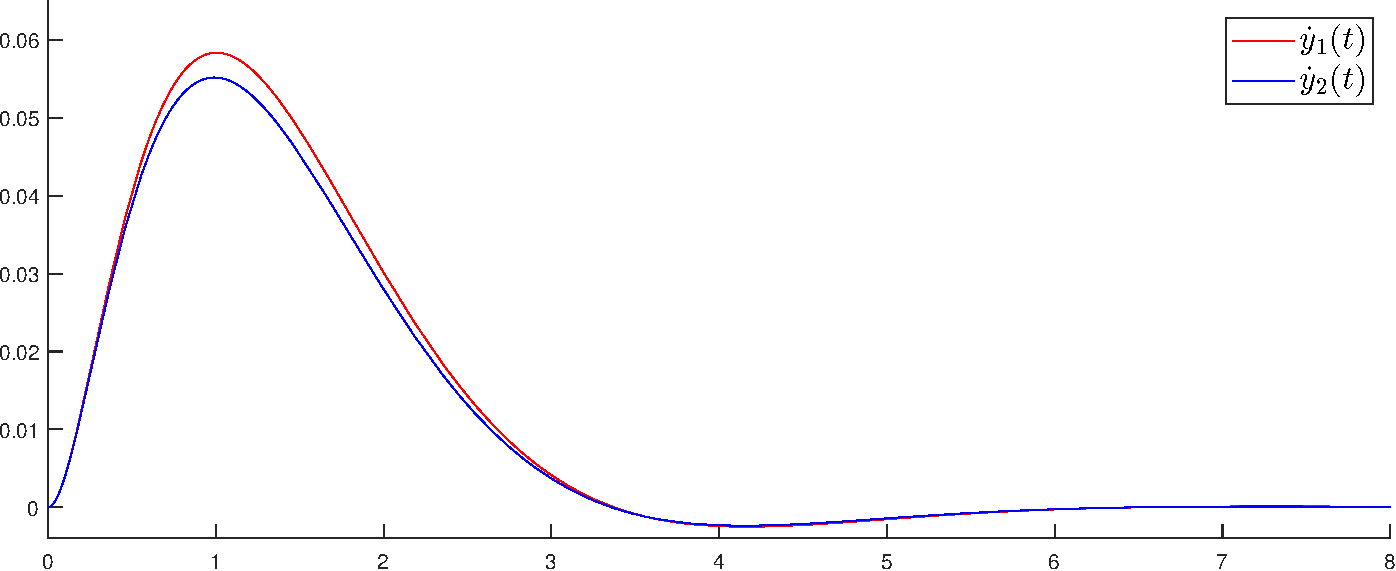
\includegraphics[width=\linewidth]{exact.pdf}
        \caption{Wykresy $\dot{y}_1(t)$, $\dot{y}_2(t)$ wyznaczonych analitycznie procedurą \texttt{dsolve} }
        \label{fig:rys1} % Optional: Use this label for referencing
    \end{figure}

    \subsection{Przekształcenie URRZ do postaci macierzowej}
    %Prawa strona URRZ \eqref{URRZ} jest liniowa względem $y_1$ oraz $y_2$, a jej zależność od czasu $t$ może być uwzględniona w wektorze wymuszenia $bx(t)bx(t)$
    Niech $ \y = \begin{bmatrix} y_1\\[1em]y_2 \end{bmatrix} $,
    wtedy $ \y' = \begin{bmatrix} \dfrac{dy_2}{dt}\\[1em]\dfrac{dy_1}{dt} \end{bmatrix} $,
    oraz niech $\mathbf{f}\left(t,\y\right) = \y'$.\\[1em]
    Wtedy URRZ \eqref{URRZ} można przedstawić następująco:
    \begin{equation}
        \label{f}
         \mathbf{f}\left(t,\y\right) = \A\y + \b x(t)
    \end{equation}
    gdzie
    $$ \A = \begin{bmatrix} -\dfrac{14}{3} & -\dfrac{2}{3}  \\[1em]\dfrac{2}{3} & -\dfrac{19}{3} \end{bmatrix} \qquad
       \b = \begin{bmatrix} 1\\1 \end{bmatrix}$$
    Funkcja $\mathbf{f}\left(t_n,\y_n\right)$ określona jest przez
    $\left. \dfrac{d\y(t)}{dt} \right|_{t=t_n} = \mathbf{f}(t_n,\y_n)$.

    \subsection{Procedura ode45}
    Za pomocą poniższego kodu korzystającego z procedury \texttt{ode45} wyznaczono rozwiązanie \eqref{URRZ}
    %\subsection*{plik \texttt{Projekt1.m}}
    \lstinputlisting[linerange={31-39}]{../Projekt1.m}
    Wykresy $\hat{y}_1(t)$ oraz $\hat{y}_2(t)$ otrzymanych procedurą \texttt{ode45} są, wraz z wynikami dokładnymi, przedstawione na \hyperref[fig:rys2]{rysunku 2.}
    \begin{figure}[H]
        \centering
        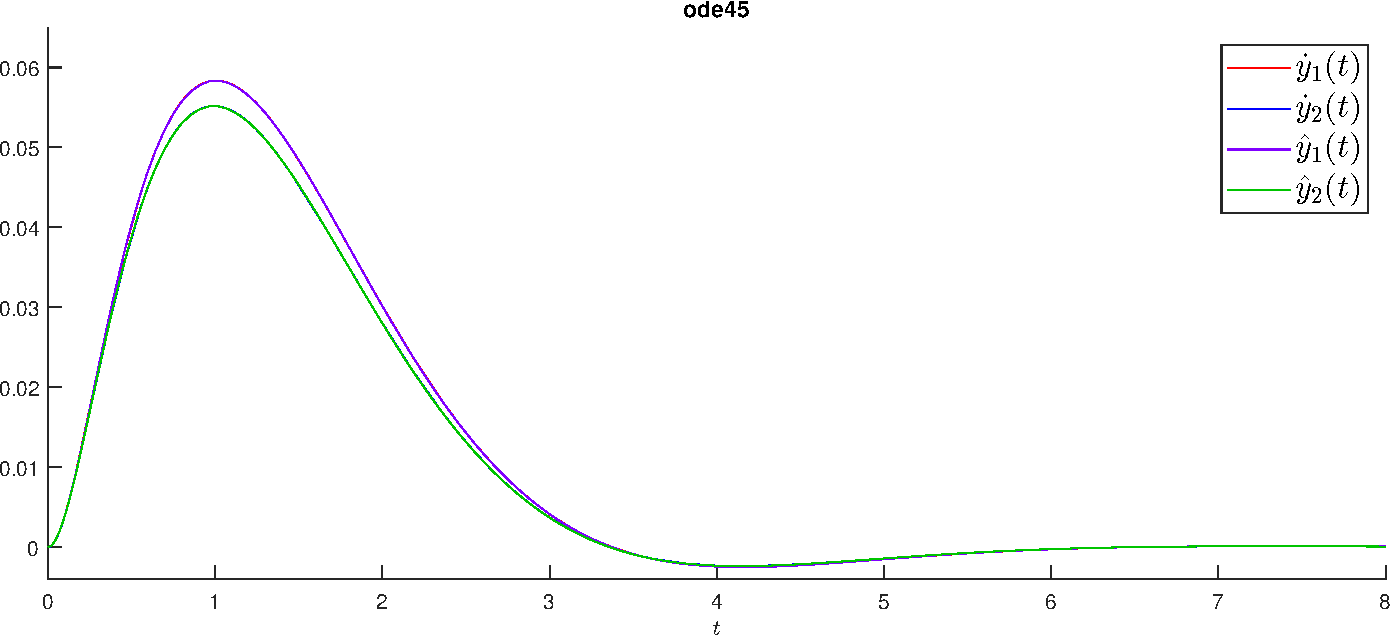
\includegraphics[width=\linewidth]{wykres1t.pdf}
        \caption{Wykresy $\dot{y}_1(t)$, $\dot{y}_2(t)$ oraz $\hat{y}_1(t)$, $\hat{y}_2(t)$ otrzymanych procedurą \texttt{ode45} }
        \label{fig:rys2} % Optional: Use this label for referencing
    \end{figure}

    \subsection{Metoda 1}
    Metoda 1. zdefiniowana jest wzorem
    \begin{equation}
        \label{m1}
        \y_n = \y_{n-1} +
        h\mathbf{f}\bigg(t_{n-1} + \dfrac{h}{2},\y_{n-1} +              \dfrac{h}{2}\mathbf{f}\big(t_{n-1},\y_{n-1}\big)\bigg)
    \end{equation}
    Podstawiając \eqref{f} do \eqref{m1} otrzymano
    $$
    \y_n = \y_{n-1} +
    h\Bigg(A\left(\y_{n-1} + \dfrac{h}{2}\Big(A\y_{n-1} + \b x(t_{n-1})\Big)\right) +
    \b x\left(t_{n-1} + \dfrac{h}{2}\right)\Bigg)
    $$
    Kod zawierający implementację metody 1.:
    %\subsection*{plik \texttt{metoda1.m}}
    \lstinputlisting{../metoda1.m}
    \noindent
    Wykresy $\hat{y}_1(t)$ oraz $\hat{y}_2(t)$ otrzymanych metodą 1. są, wraz z wynikami dokładnymi, przedstawione na \hyperref[fig:rys3]{rysunku 3.}
    \begin{figure}[H]
        \centering
        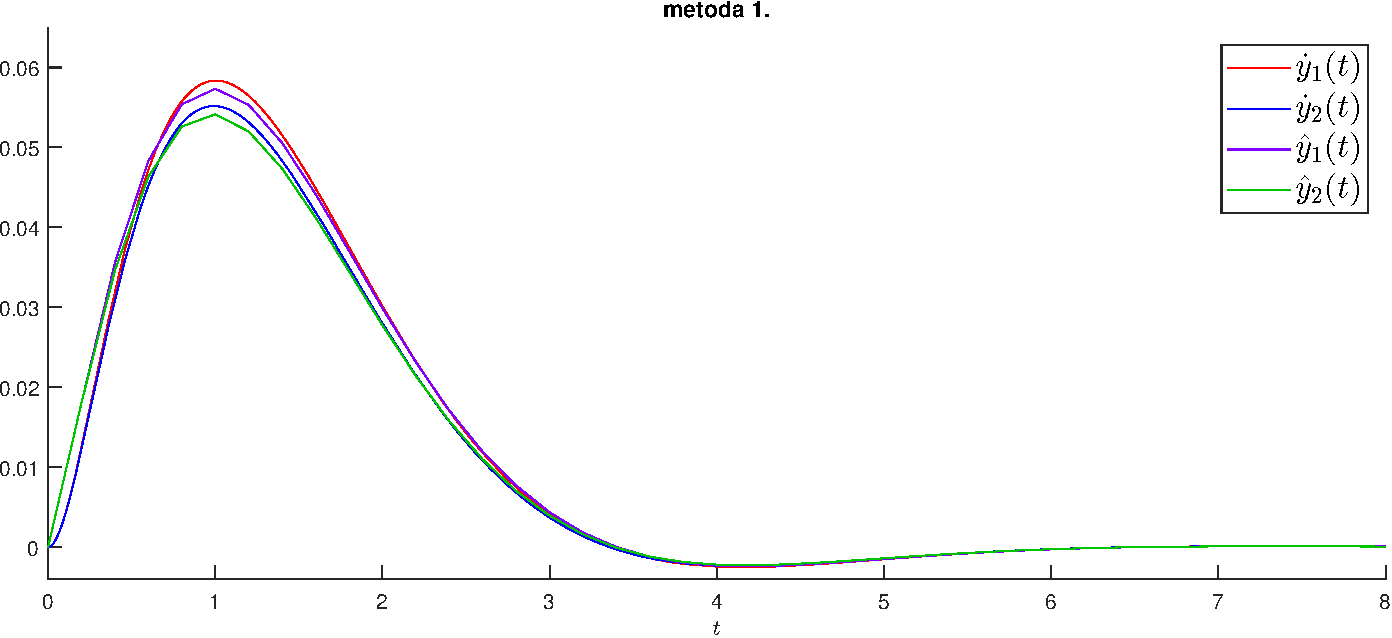
\includegraphics[width=\linewidth]{wykres2t.pdf}
        \caption{Wykresy $\dot{y}_1(t)$, $\dot{y}_2(t)$ oraz $\hat{y}_1(t)$, $\hat{y}_2(t)$ otrzymanych metodą 1. dla kroku $h = 0.2$ }
        \label{fig:rys3} % Optional: Use this label for referencing
    \end{figure}

    \newpage
    \subsection{Metoda 2}
    Metoda 2. jest metodą niejawną zdefiniowaną wzorem
    \begin{equation}
        \label{m2}
        \y_n = \y_{n-2} + h\Big[\mathbf{f}\left(t_{n},\y_{n}\right) +       \mathbf{f}\left(t_{n-2},\y_{n-2}\right)\Big]
    \end{equation}
    Podstawiając \eqref{f} do \eqref{m2} otrzymano
    $$ \y_n = \y_{n-2} + h\Big[\big(\A\y_n + \b x(t_n) \big) + \big(\A\y_{n-2} + \b x(t_{n-2})\big)\Big] $$
    Po przekształceniach
    $$ \y_n = \Big( \I - h \A \Big)^{-1} \Big( \y_{n-2} + h\A\y_{n-2} + h\b x(t_n) + h\b x(t_{n-2}) \Big) $$
    W celu wyznaczenia $\y_2$ zastosowano niejawną metodę Eulera ($\y_1$ to zerowy warunek początkowy)
    $$ \y_2 = \Big(\I - h\A\Big)^{-1} \Big(\y_1 + h\b x(t_2)\Big) $$
    Kod zawierający implementację metody 2.:
    %\subsection*{plik \texttt{metoda2.m}}
    \lstinputlisting{../metoda2.m}
    \noindent
    Wykresy $\hat{y}_1(t)$ oraz $\hat{y}_2(t)$ otrzymanych metodą 2. są, wraz z wynikami dokładnymi, przedstawione na \hyperref[fig:rys4]{rysunku 4.}
    \begin{figure}[H]
        \centering
        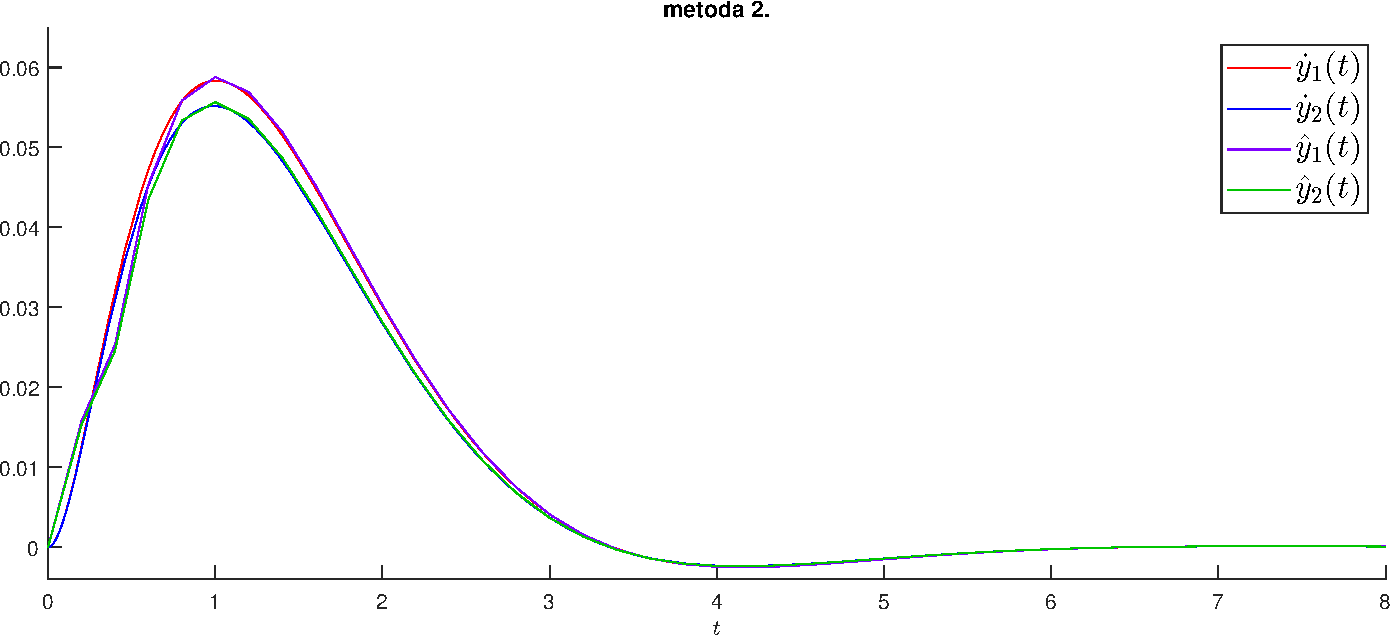
\includegraphics[width=\linewidth]{wykres3t.pdf}
        \caption{Wykresy $\dot{y}_1(t)$, $\dot{y}_2(t)$ oraz $\hat{y}_1(t)$, $\hat{y}_2(t)$ otrzymanych metodą 2. dla kroku $h = 0.2$ }
        \label{fig:rys4} % Optional: Use this label for referencing
    \end{figure}

    \subsection{Metoda 3}
    Metoda 3. zdefiniowana jest wzorem
    \begin{equation}
        \label{m3}
        \y_n = \y_{n-1} + h\sum\limits_{k=1}^{3}w_k\mathbf{f}_k
    \end{equation}
    Po rozpisaniu sumy
    \begin{equation}
        \label{m3rozpisane}
        \y_n = \y_{n-1} + h\Big( w_1\f_1 + w_2\f_2 + w_3\f_3 \Big)
    \end{equation}
    gdzie
    \begin{equation}
        \label{fk}
        \mathbf{f}_k = \mathbf{f}\bigg(t_{n-1}+c_kh,\y_{n-1} + h\sum\limits_{\kappa=1}^{3}a_{k,\kappa}\mathbf{f}_\kappa\bigg)
    \end{equation}
    a współczynniki przyjmują wartości przedstawione w poniższej tabeli Butchera:
    \begin{center}
        $\arraycolsep=5pt\def\arraystretch{1.5}
        \begin{array}{c|ccc}
            c_1 & a_{1,1} & a_{1,2} & a_{1,3} \\
            c_2 & a_{2,1} & a_{2,2} & a_{2,3} \\
            c_3 & a_{3,1} & a_{3,2} & a_{3,3} \\
            \hline
            & w_1 & w_2 & w_3
        \end{array}
        \hspace{1cm} = \hspace{1cm}
        \begin{array}{c|ccc}
            0            & \frac{1}{6} & -\frac{1}{6} & 0 \\
            \dfrac{1}{2} & \frac{1}{6} & \frac{1}{3} & 0 \\
            1            & \frac{1}{6} & \frac{5}{6} & 0 \\
            \hline
            & \frac{1}{6} & \frac{2}{3} & \frac{1}{6}
        \end{array} $
    \end{center}
    Z \eqref{fk} otrzymano
    \begin{equation}
        \label{uklad1}
        \left\{\begin{array}{c}
            \begin{aligned}
                \f_1 &= \A\big(\y_{n-1} + ha_{1,1}\f_1 + ha_{1,2}\f_2 +   ha_{1,3}\f_3\big) + \b x\big(t_{n-1} + c_1h \big) \\
                \f_2 &= \A\big(\y_{n-1} + ha_{2,1}\f_1 + ha_{2,2}\f_2 +   ha_{2,3}\f_3\big) + \b x\big(t_{n-1} + c_2h \big) \\
                \f_3 &= \A\big(\y_{n-1} + ha_{3,1}\f_1 + ha_{3,2}\f_2 +   ha_{3,3}\f_3\big) + \b x\big(t_{n-1} + c_3h \big) \\
            \end{aligned}
        \end{array}\right.
    \end{equation}
    Przekształcając \eqref{uklad1} otrzymano
    \begin{equation}
        \label{uklad2}
        \left\{\begin{array}{c}
            \begin{aligned}
                \big(\I - ha_{1,1}\A\big)\f_1 \hspace{0.8em} &- \hspace{1cm} ha_{1,2}\A\f_2   &- \hspace{1cm} ha_{1,3}\A\f_3    &= \A\y_{n-1} + \b x\big(t_{n-1} + c_1h\big)\\
                -ha_{2,1}\A\f_1               \hspace{0.8em} &+ \big(\I - ha_{2,2}\A\big)\f_2 &- \hspace{1cm} ha_{1,3}\A\f_3    &= \A\y_{n-1} + \b x\big(t_{n-1} + c_2h\big)\\
                -ha_{3,1}\A\f_1               \hspace{0.8em} &- \hspace{1cm} ha_{3,2}\A\f_2   &+ \big(\I - ha_{3,3}\A\big)\f_3  &= \A\y_{n-1} + \b x\big(t_{n-1} + c_3h\big)\\
            \end{aligned}
        \end{array}\right.
    \end{equation}
    Układ \eqref{uklad2} można przedstawić w następującej postaci:
    \begin{equation}
        \label{uklad}
        \mathbf{L}\mathbf{g} = \mathbf{p}
    \end{equation}
    gdzie
    $$
    \mathbf{g} = \begin{bmatrix} \f_1 \\ \f_2 \\ \f_3 \end{bmatrix} \qquad
    \mathbf{L} = \begin{bmatrix*}[r]
        \I - ha_{1,1}\A & -ha_{1,2}\A     & -ha_{1,3}\A   \\
        -ha_{2,1}\A     & \I - ha_{2,2}\A & -ha_{2,3}\A   \\
        -ha_{3,1}\A     & -ha_{3,2}\A     & \I - ha_{3,3}\A \\
    \end{bmatrix*} \qquad
    \mathbf{p} = \begin{bmatrix*}[r]
        \A\y_{n-1} + \b x\big(t_{n-1} + c_1h\big)\\
        \A\y_{n-1} + \b x\big(t_{n-1} + c_2h\big)\\
        \A\y_{n-1} + \b x\big(t_{n-1} + c_3h\big)\\
    \end{bmatrix*}
    $$
    Rozwiązując układ \eqref{uklad} wyznaczono $\f_1$, $\f_2$ oraz $\f_3$.
    Następnie podstawiono otrzymane $\f_i$ do \eqref{m3rozpisane} w celu wyliczenia $\y_n$ dla $n \geqslant 2$.
    \newpage
    \noindent Kod zawierający implementację metody 3.:
    %\subsection*{plik \texttt{metoda3.m}}
    \lstinputlisting{../metoda3.m}
    \noindent
    Wykresy $\hat{y}_1(t)$ oraz $\hat{y}_2(t)$ otrzymanych metodą 3. są, wraz z wynikami dokładnymi, przedstawione na \hyperref[fig:rys5]{rysunku 5.}
    \begin{figure}[H]
        \centering
        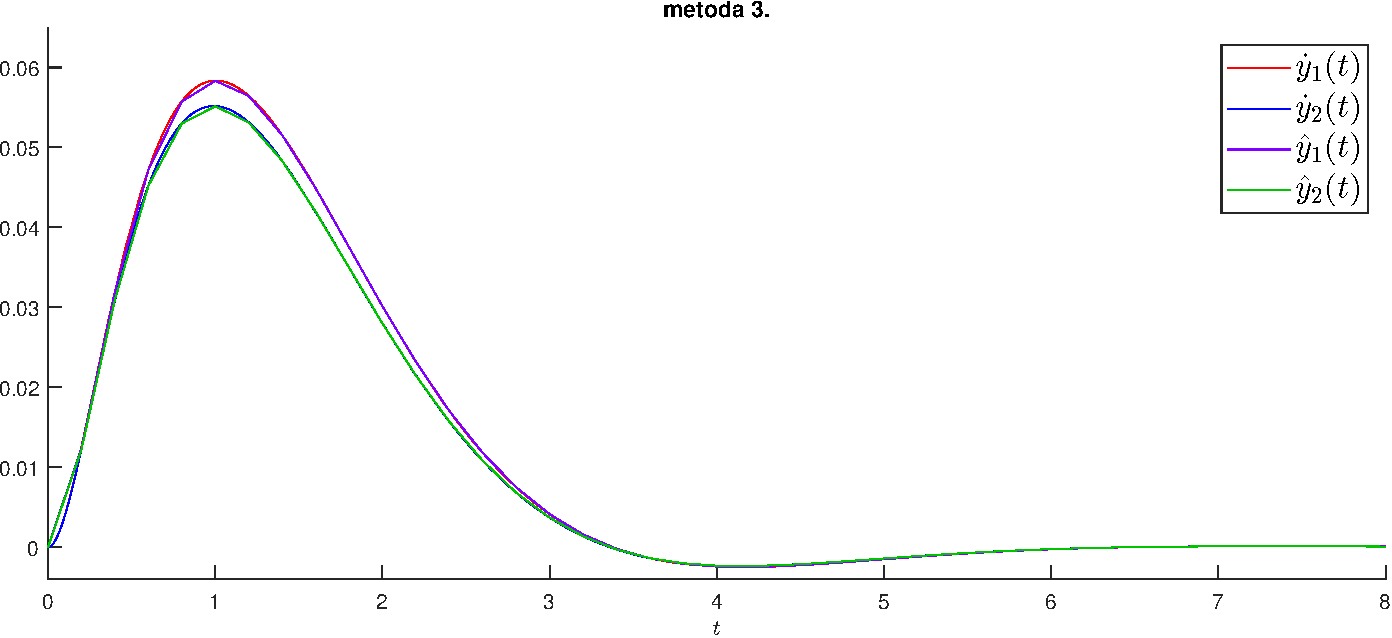
\includegraphics[width=\linewidth]{wykres4t.pdf}
        \caption{Wykresy $\dot{y}_1(t)$, $\dot{y}_2(t)$ oraz $\hat{y}_1(t)$, $\hat{y}_2(t)$ otrzymanych metodą 3. dla kroku $h = 0.2$ }
        \label{fig:rys5} % Optional: Use this label for referencing
    \end{figure}

    \newpage
    % Dyskusja wyników eksperymentów numerycznych
    \section{Dyskusja Wyników Eksperymentów Numerycznych}
    W ramach przeprowadzonego rozwiązywania układu równań różniczkowych zwyczajnych (URRZ) \eqref{URRZ}
    uzyskano wartości funkcji $y_1(t)$ oraz $y_2(t)$ dla pięciu różnych podejść:
    analitycznego, wykorzystującego procedurę \texttt{dsolve}, oraz czterech metod numerycznych,
    w tym procedury \texttt{ode45} oraz trzech innych metod dyskretnych określonych jako metoda 1, metoda 2 i metoda 3.
    \\\par\noindent
    Wyniki uzyskane przy pomocy procedury ode45 wykazały niemal dokładną zgodność z rozwiązaniem analitycznym.
    Jest to zgodne z teoretycznym założeniem, że ode45, jako metoda adaptacyjna oparta na algorytmie Rungego-Kutty czwartego i piątego rzędu,
    charakteryzuje się wysoką precyzją w przypadkach, gdzie funkcje są wystarczająco gładkie.
    Wykresy $\dot{y}_1(t)$ i $\hat{y}_1(t)$ oraz $\dot{y}_2(t)$ i $\hat{y}_2(t)$ nałożone na siebie w tych przypadkach niemalże się pokrywają.
    \\\par\noindent
    Trzy ostatnie metody okazały się zauważalnie mniej dokładne, z czego metoda 1. jest widocznie mniej dokładna niż metody 2. i 3.,
    a metoda 3. wydaje się być dokładniejsza od metody 2., gdyż na wykresach przedstawionych na \hyperref[fig:rys5]{rysunku 5.}
    wyliczone punkty pokrywają się z rozwiązaniem dokładnym częściej niż w przypadku metody 2. na \hyperref[fig:rys5]{rysunku 4}.
    \\\par\noindent
    W celu jednoznacznego ustalenia, która metoda daje najdokładniejsze rozwiązania,
    zbadano zależność dokładności rozwiązań numerycznych uzyskanych za ich pomocą od długości kroku całkowania $h$, dla $h \in \big[0.01, 1.00\big]$.
    Jako kryterium dokładności rozwiązań przyjęto zagregowane błędy względne zdefiniowane następująco:
    $$
    \delta_1(h) = \dfrac
    {\sum_{n=1}^{N(h)}\bigg( \hat{y}_1\Big(t_n,h\Big) - \dot{y}_1\Big(t_n\Big) \bigg)^2}
    {\sum_{n=1}^{N(h)}\bigg(\dot{y}_1\Big(t_n\Big)\bigg)^2}
    \qquad \text{i} \qquad
    \delta_2(h) = \dfrac
    {\sum_{n=1}^{N(h)}\bigg( \hat{y}_2\Big(t_n,h\Big) - \dot{y}_2\Big(t_n\Big) \bigg)^2}
    {\sum_{n=1}^{N(h)}\bigg(\dot{y}_2\Big(t_n\Big)\bigg)^2}
    $$
    gdzie $\dot{y}_1(t_n)$ i $\dot{y}_2(t_n)$ to wartości funkcji uzyskanych analitycznie za pomocą procedury \texttt{dsolve},
    a $\hat{y}_1(t_n,h)$ i $\hat{y}_2(t_n,h)$ to ich estymaty uzyskane dla kroku całkowania $h$ numeryczną metodą dyskretną.
    $N(h)$ oznacza zależną od kroku całkowania liczbę punktów rozwiązania.
    \\\par\noindent
    Zależność $ \delta_1(h) $ od $h$ dla trzech ostatnich metod została przedstawiona na \hyperref[fig:delta1]{rysunku 6.}
    \begin{figure}[h]
        \centering
        \label{fig:delta1}
        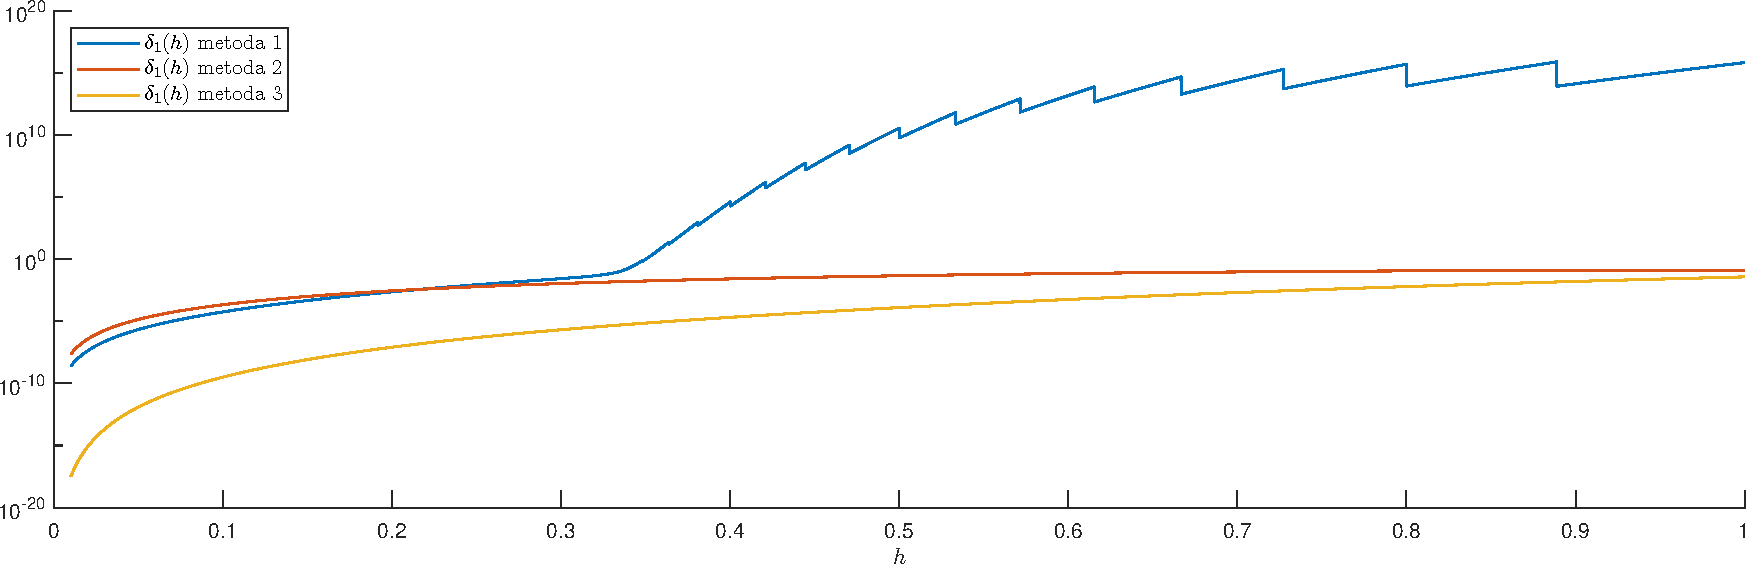
\includegraphics[width=\linewidth]{delta1new.pdf}
        \caption{Wykresy $\delta_1(h)$ dla metod 1.,2.,3. }
    \end{figure}
    \newpage
    \noindent
    Zależność $ \delta_2(h) $ od $h$ dla trzech ostatnich metod została przedstawiona na \hyperref[fig:delta2]{rysunku 7.}
    \begin{figure}[H]
        \centering
        \label{fig:delta2}
        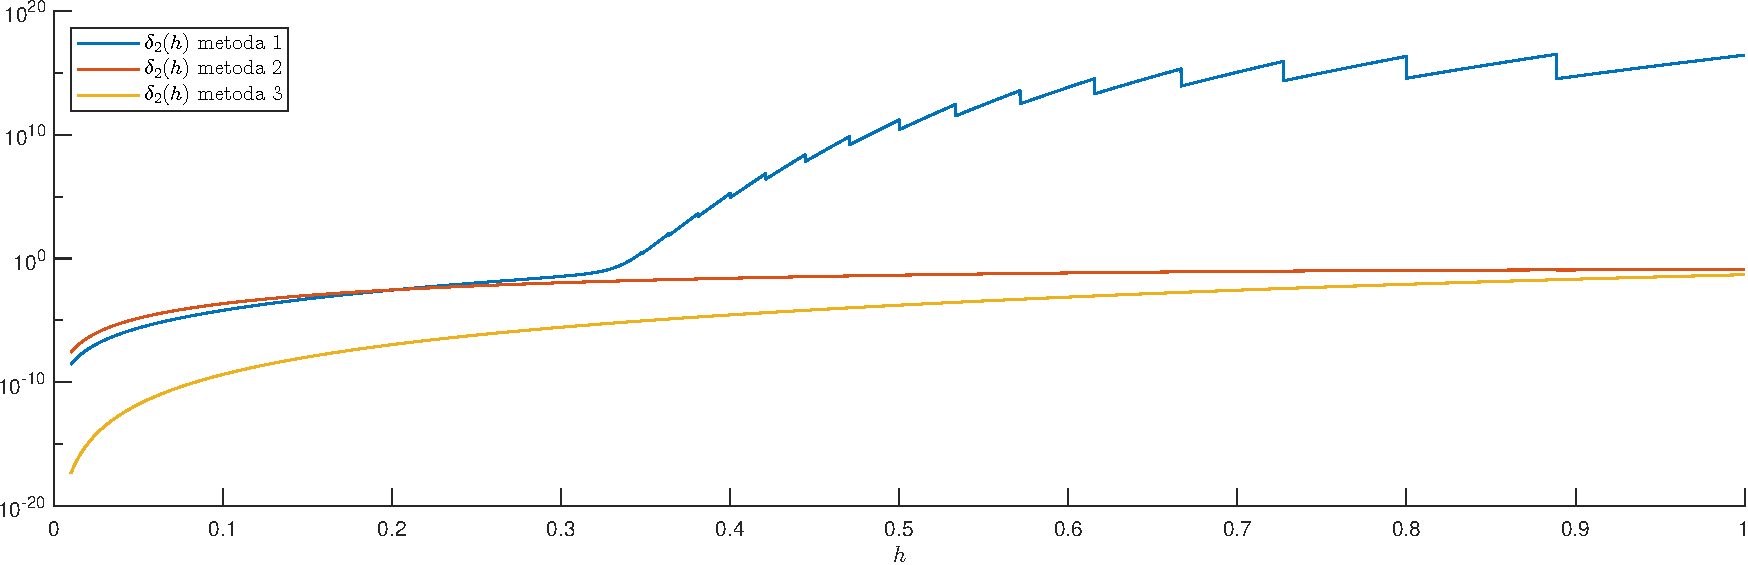
\includegraphics[width=\linewidth]{delta2new.pdf}
        \caption{Wykresy $\delta_2(h)$ dla metod 1.,2.,3. }
    \end{figure}

    \noindent
    Na podstawie \hyperref[fig:delta1]{rysunku 6.} oraz \hyperref[fig:delta2]{rysunku 7.} zaobserwowano,
    że metoda 3. jest najdokładniejsza spośród trzech testowanych metod,
    a metoda 2. jest dokładniejsza od metody 1 dla $h$ większych niż $h \approx 0.2$.
    Dla metody 1. zaobserwowano zjawisko niestabilności numerycznej.
    Dla $h$ większych niż $h \approx \frac{1}{3}$ tempo wzrostu $\delta_1(h)$ i $\delta_2(h)$ znacznie rośnie, dokładność metody 1. znacznie się pogarsza.

    \newpage

    % Lista źródeł informacji
    \section*{Bibliografia}
    \addcontentsline{toc}{section}{Bibliografia}
    \begin{enumerate}
        \item Dokumentacja MATLAB: \url{https://www.mathworks.com/help/matlab}.
    \end{enumerate}

    \newpage

    % Listing opracowanych programów
    \section*{Listing Programów}
    \addcontentsline{toc}{section}{Listing Programów}

    \subsection*{plik \texttt{Projekt1.m}}
    \lstinputlisting{../Projekt1.m}
    \newpage
    \subsection*{plik \texttt{solve\_using\_dsolve.m}}
    \lstinputlisting{../solve_using_dsolve.m}
    \subsection*{plik \texttt{plot\_exact.m}}
    \lstinputlisting{../plot_exact.m}
    \subsection*{plik \texttt{metoda1.m}}
    \lstinputlisting{../metoda1.m}
    \newpage
    \subsection*{plik \texttt{metoda2.m}}
    \lstinputlisting{../metoda2.m}
    \subsection*{plik \texttt{metoda3.m}}
    \lstinputlisting{../metoda3.m}
    \newpage
    \subsection*{plik \texttt{plot\_results.m}}
    \lstinputlisting{../plot_results.m}
    \subsection*{plik \texttt{calculate\_error.m}}
    \lstinputlisting{../calculate_error.m}

\end{document}
